\documentclass[twoside]{book}

% Packages required by doxygen
\usepackage{fixltx2e}
\usepackage{calc}
\usepackage{doxygen}
\usepackage[export]{adjustbox} % also loads graphicx
\usepackage{graphicx}
\usepackage[utf8]{inputenc}
\usepackage{makeidx}
\usepackage{multicol}
\usepackage{multirow}
\PassOptionsToPackage{warn}{textcomp}
\usepackage{textcomp}
\usepackage[nointegrals]{wasysym}
\usepackage[table]{xcolor}

% Font selection
\usepackage[T1]{fontenc}
\usepackage[scaled=.90]{helvet}
\usepackage{courier}
\usepackage{amssymb}
\usepackage{sectsty}
\renewcommand{\familydefault}{\sfdefault}
\allsectionsfont{%
  \fontseries{bc}\selectfont%
  \color{darkgray}%
}
\renewcommand{\DoxyLabelFont}{%
  \fontseries{bc}\selectfont%
  \color{darkgray}%
}
\newcommand{\+}{\discretionary{\mbox{\scriptsize$\hookleftarrow$}}{}{}}

% Page & text layout
\usepackage{geometry}
\geometry{%
  a4paper,%
  top=2.5cm,%
  bottom=2.5cm,%
  left=2.5cm,%
  right=2.5cm%
}
\tolerance=750
\hfuzz=15pt
\hbadness=750
\setlength{\emergencystretch}{15pt}
\setlength{\parindent}{0cm}
\setlength{\parskip}{3ex plus 2ex minus 2ex}
\makeatletter
\renewcommand{\paragraph}{%
  \@startsection{paragraph}{4}{0ex}{-1.0ex}{1.0ex}{%
    \normalfont\normalsize\bfseries\SS@parafont%
  }%
}
\renewcommand{\subparagraph}{%
  \@startsection{subparagraph}{5}{0ex}{-1.0ex}{1.0ex}{%
    \normalfont\normalsize\bfseries\SS@subparafont%
  }%
}
\makeatother

% Headers & footers
\usepackage{fancyhdr}
\pagestyle{fancyplain}
\fancyhead[LE]{\fancyplain{}{\bfseries\thepage}}
\fancyhead[CE]{\fancyplain{}{}}
\fancyhead[RE]{\fancyplain{}{\bfseries\leftmark}}
\fancyhead[LO]{\fancyplain{}{\bfseries\rightmark}}
\fancyhead[CO]{\fancyplain{}{}}
\fancyhead[RO]{\fancyplain{}{\bfseries\thepage}}
\fancyfoot[LE]{\fancyplain{}{}}
\fancyfoot[CE]{\fancyplain{}{}}
\fancyfoot[RE]{\fancyplain{}{\bfseries\scriptsize Generated by Doxygen }}
\fancyfoot[LO]{\fancyplain{}{\bfseries\scriptsize Generated by Doxygen }}
\fancyfoot[CO]{\fancyplain{}{}}
\fancyfoot[RO]{\fancyplain{}{}}
\renewcommand{\footrulewidth}{0.4pt}
\renewcommand{\chaptermark}[1]{%
  \markboth{#1}{}%
}
\renewcommand{\sectionmark}[1]{%
  \markright{\thesection\ #1}%
}

% Indices & bibliography
\usepackage{natbib}
\usepackage[titles]{tocloft}
\setcounter{tocdepth}{3}
\setcounter{secnumdepth}{5}
\makeindex

% Custom commands
\newcommand{\clearemptydoublepage}{%
  \newpage{\pagestyle{empty}\cleardoublepage}%
}

\usepackage{caption}
\captionsetup{labelsep=space,justification=centering,font={bf},singlelinecheck=off,skip=4pt,position=top}

%===== C O N T E N T S =====

\begin{document}

% Titlepage & ToC
\pagenumbering{alph}
\begin{titlepage}
\vspace*{7cm}
\begin{center}%
{\Large P\+A5 }\\
\vspace*{1cm}
{\large Generated by Doxygen 1.8.13}\\
\end{center}
\end{titlepage}
\clearemptydoublepage
\pagenumbering{roman}
\tableofcontents
\clearemptydoublepage
\pagenumbering{arabic}

%--- Begin generated contents ---
\chapter{Hierarchical Index}
\section{Class Hierarchy}
This inheritance list is sorted roughly, but not completely, alphabetically\+:\begin{DoxyCompactList}
\item \contentsline{section}{Organism}{\pageref{classOrganism}}{}
\begin{DoxyCompactList}
\item \contentsline{section}{Ant}{\pageref{classAnt}}{}
\item \contentsline{section}{Doodlebug}{\pageref{classDoodlebug}}{}
\end{DoxyCompactList}
\end{DoxyCompactList}

\chapter{Class Index}
\section{Class List}
Here are the classes, structs, unions and interfaces with brief descriptions\+:\begin{DoxyCompactList}
\item\contentsline{section}{\textbf{ Compare\+Events} }{\pageref{structCompareEvents}}{}
\item\contentsline{section}{\textbf{ Customer} \\*\doxyref{Customer}{p.}{classCustomer} is a derived \doxyref{Event}{p.}{classEvent} class that contains information on how long a customer was in the bank for }{\pageref{classCustomer}}{}
\item\contentsline{section}{\textbf{ Event} \\*\doxyref{Event}{p.}{classEvent} is an abstract class that contains the time an event occurs at }{\pageref{classEvent}}{}
\item\contentsline{section}{\textbf{ Event\+Queue} \\*\doxyref{Event\+Queue}{p.}{classEventQueue} is a priorty\+\_\+queue of events, is the global overhead for the entire project }{\pageref{classEventQueue}}{}
\item\contentsline{section}{\textbf{ Teller} \\*\doxyref{Teller}{p.}{classTeller} is the derived class of \doxyref{Event}{p.}{classEvent} that carries additional info such as idle\+\_\+time for each specific teller }{\pageref{classTeller}}{}
\item\contentsline{section}{\textbf{ Teller\+Queue} \\*\doxyref{Teller\+Queue}{p.}{classTellerQueue} is a derived class from \doxyref{Event\+Queue}{p.}{classEventQueue} that does nothing extra, it only holds \doxyref{Customer}{p.}{classCustomer} objects though }{\pageref{classTellerQueue}}{}
\end{DoxyCompactList}

\chapter{File Index}
\section{File List}
Here is a list of all files with brief descriptions\+:\begin{DoxyCompactList}
\item\contentsline{section}{\textbf{ Ant.\+cpp} }{\pageref{Ant_8cpp}}{}
\item\contentsline{section}{\textbf{ Ant.\+h} }{\pageref{Ant_8h}}{}
\item\contentsline{section}{\textbf{ Doodlebug.\+cpp} }{\pageref{Doodlebug_8cpp}}{}
\item\contentsline{section}{\textbf{ Doodlebug.\+h} }{\pageref{Doodlebug_8h}}{}
\item\contentsline{section}{\textbf{ main.\+cpp} }{\pageref{main_8cpp}}{}
\item\contentsline{section}{\textbf{ main.\+h} }{\pageref{main_8h}}{}
\item\contentsline{section}{\textbf{ Organism.\+cpp} }{\pageref{Organism_8cpp}}{}
\item\contentsline{section}{\textbf{ Organism.\+h} }{\pageref{Organism_8h}}{}
\end{DoxyCompactList}

\chapter{Class Documentation}
\section{Ant Class Reference}
\label{classAnt}\index{Ant@{Ant}}


{\ttfamily \#include $<$Ant.\+h$>$}

Inheritance diagram for Ant\+:\begin{figure}[H]
\begin{center}
\leavevmode
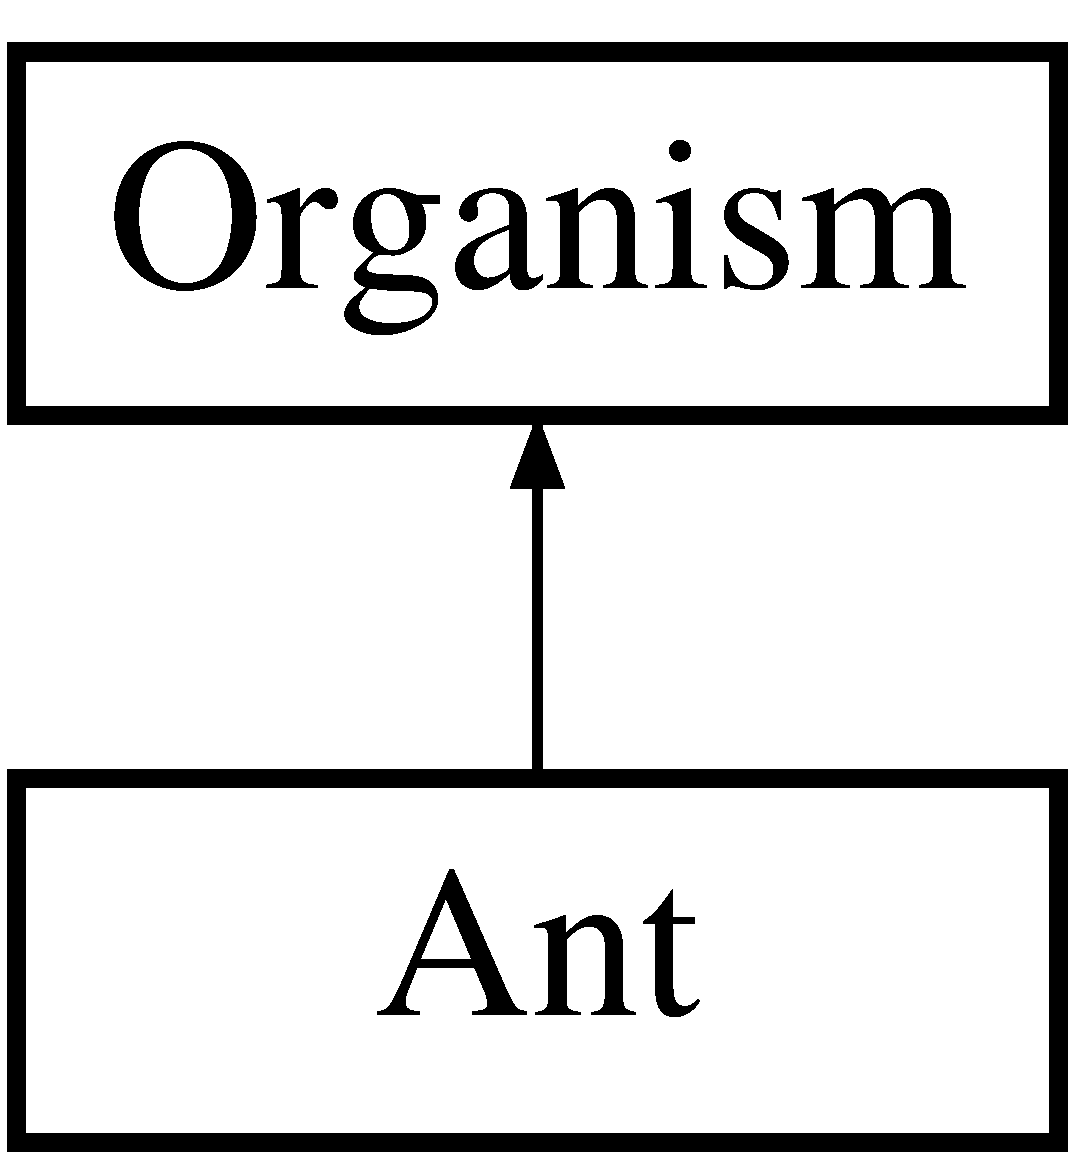
\includegraphics[height=2.000000cm]{classAnt}
\end{center}
\end{figure}
\subsection*{Public Member Functions}
\begin{DoxyCompactItemize}
\item 
\textbf{ Ant} ()
\item 
\textbf{ Ant} (int \textbf{ x}, int \textbf{ y})
\item 
virtual \textbf{ $\sim$\+Ant} ()
\item 
int \textbf{ get\+Time} ()
\item 
void \textbf{ move} ()
\item 
\textbf{ Ant} $\ast$ \textbf{ breed} ()
\item 
bool \textbf{ is\+Move} (int \textbf{ x}, int \textbf{ y})
\item 
void \textbf{ action} ()
\end{DoxyCompactItemize}
\subsection*{Additional Inherited Members}


\subsection{Constructor \& Destructor Documentation}
\mbox{\label{classAnt_ad6c1a8f70419877f7a3e2c9c557f913d}} 
\index{Ant@{Ant}!Ant@{Ant}}
\index{Ant@{Ant}!Ant@{Ant}}
\subsubsection{Ant()\hspace{0.1cm}{\footnotesize\ttfamily [1/2]}}
{\footnotesize\ttfamily Ant\+::\+Ant (\begin{DoxyParamCaption}{ }\end{DoxyParamCaption})}

\doxyref{Ant()}{p.}{classAnt_ad6c1a8f70419877f7a3e2c9c557f913d} is the constructor for an \doxyref{Ant}{p.}{classAnt} object with no parameters 

Referenced by breed().

\mbox{\label{classAnt_a4f1a3a8388155501d0b2debffc1cbc70}} 
\index{Ant@{Ant}!Ant@{Ant}}
\index{Ant@{Ant}!Ant@{Ant}}
\subsubsection{Ant()\hspace{0.1cm}{\footnotesize\ttfamily [2/2]}}
{\footnotesize\ttfamily Ant\+::\+Ant (\begin{DoxyParamCaption}\item[{int}]{x,  }\item[{int}]{y }\end{DoxyParamCaption})}

\doxyref{Ant()}{p.}{classAnt_ad6c1a8f70419877f7a3e2c9c557f913d} is the constructor for an \doxyref{Ant}{p.}{classAnt} object with coordinates as parameters, and is initialized with default values. It icrements the count of total and current ants 

References Organism\+::age, Organism\+::is\+Prey, numA, totalA, Organism\+::x, and Organism\+::y.

\mbox{\label{classAnt_a33ca6bd592236726a18a2159908e4116}} 
\index{Ant@{Ant}!````~Ant@{$\sim$\+Ant}}
\index{````~Ant@{$\sim$\+Ant}!Ant@{Ant}}
\subsubsection{$\sim$\+Ant()}
{\footnotesize\ttfamily Ant\+::$\sim$\+Ant (\begin{DoxyParamCaption}{ }\end{DoxyParamCaption})\hspace{0.3cm}{\ttfamily [virtual]}}

\doxyref{$\sim$\+Ant()}{p.}{classAnt_a33ca6bd592236726a18a2159908e4116} is the destructor for an \doxyref{Ant}{p.}{classAnt} object, it decrements the number of current ants 

References numA.



\subsection{Member Function Documentation}
\mbox{\label{classAnt_a39fabe2c96298d5f7beb86649bf2dcab}} 
\index{Ant@{Ant}!action@{action}}
\index{action@{action}!Ant@{Ant}}
\subsubsection{action()}
{\footnotesize\ttfamily void Ant\+::action (\begin{DoxyParamCaption}{ }\end{DoxyParamCaption})\hspace{0.3cm}{\ttfamily [virtual]}}

\doxyref{action()}{p.}{classAnt_a39fabe2c96298d5f7beb86649bf2dcab} processes a regular turn of an ant, moving the ant and checking if it can breed in the current turn 

Implements \textbf{ Organism} \doxyref{}{p.}{classOrganism_af4dd34a96becf4f02ce4597901b81f60}.



References Organism\+::age, breed(), Organism\+::can\+Move, move(), Organism\+::x, and Organism\+::y.

\mbox{\label{classAnt_a6829e25685f8a52a2acc38f5edbfc549}} 
\index{Ant@{Ant}!breed@{breed}}
\index{breed@{breed}!Ant@{Ant}}
\subsubsection{breed()}
{\footnotesize\ttfamily \textbf{ Ant} $\ast$ Ant\+::breed (\begin{DoxyParamCaption}{ }\end{DoxyParamCaption})\hspace{0.3cm}{\ttfamily [virtual]}}

\doxyref{breed()}{p.}{classAnt_a6829e25685f8a52a2acc38f5edbfc549} checks the age of the ant and creates a new ant if the age of the ant is at least 3. Upon creating a new ant, moves it into an adjacent cell and resets the age of the current ant

\begin{DoxyReturn}{Returns}
pointer to the newly born ant or a null object if breeding conditions are not met 
\end{DoxyReturn}


Implements \textbf{ Organism} \doxyref{}{p.}{classOrganism_ad963420d8437f87bd8fe4277cc7f810a}.



References Organism\+::age, Ant(), move(), totalA, Organism\+::x, and Organism\+::y.



Referenced by action().

\mbox{\label{classAnt_a39712b5c8852fcf2f0b7857e276e95c7}} 
\index{Ant@{Ant}!get\+Time@{get\+Time}}
\index{get\+Time@{get\+Time}!Ant@{Ant}}
\subsubsection{get\+Time()}
{\footnotesize\ttfamily int Ant\+::get\+Time (\begin{DoxyParamCaption}{ }\end{DoxyParamCaption})\hspace{0.3cm}{\ttfamily [virtual]}}

\doxyref{get\+Time()}{p.}{classAnt_a39712b5c8852fcf2f0b7857e276e95c7} is a getter function for the turns which the ant has been alive

\begin{DoxyReturn}{Returns}
age of the \doxyref{Ant}{p.}{classAnt} object 
\end{DoxyReturn}


Implements \textbf{ Organism} \doxyref{}{p.}{classOrganism_a9bc6dfde09d0e18a628cf843bb037d4b}.



References Organism\+::age.

\mbox{\label{classAnt_a90943e89be8e68321ef0626e7770da59}} 
\index{Ant@{Ant}!is\+Move@{is\+Move}}
\index{is\+Move@{is\+Move}!Ant@{Ant}}
\subsubsection{is\+Move()}
{\footnotesize\ttfamily bool Ant\+::is\+Move (\begin{DoxyParamCaption}\item[{int}]{x,  }\item[{int}]{y }\end{DoxyParamCaption})\hspace{0.3cm}{\ttfamily [virtual]}}

\doxyref{is\+Move()}{p.}{classAnt_a90943e89be8e68321ef0626e7770da59} checks the state of the given cell to see whether the object can be moved into by an existing \doxyref{Ant}{p.}{classAnt}

\begin{DoxyReturn}{Returns}
a boolean for if the cell can be moved into 
\end{DoxyReturn}


Implements \textbf{ Organism} \doxyref{}{p.}{classOrganism_a7930747968e8533164d068be96f21ca0}.



References Organism\+::x, and Organism\+::y.



Referenced by move().

\mbox{\label{classAnt_aaec1e3edaddd5e0ceedc333a9ac57a4c}} 
\index{Ant@{Ant}!move@{move}}
\index{move@{move}!Ant@{Ant}}
\subsubsection{move()}
{\footnotesize\ttfamily void Ant\+::move (\begin{DoxyParamCaption}{ }\end{DoxyParamCaption})\hspace{0.3cm}{\ttfamily [virtual]}}

\doxyref{move()}{p.}{classAnt_aaec1e3edaddd5e0ceedc333a9ac57a4c} attempts to move an ant into an adjacent cell, choosing one randomly and trying the rest. If none of the cases which were tried work, \doxyref{move()}{p.}{classAnt_aaec1e3edaddd5e0ceedc333a9ac57a4c} calls itself recursively to try again. It also checks whether it is on the edge of the grid, and terminates if the ant is unable to move 

Implements \textbf{ Organism} \doxyref{}{p.}{classOrganism_a7fe2c98ea7b292d414b19bd67e885b55}.



References grid\+Len, is\+Move(), on\+Edge(), Organism\+::x, and Organism\+::y.



Referenced by action(), and breed().



The documentation for this class was generated from the following files\+:\begin{DoxyCompactItemize}
\item 
\textbf{ Ant.\+h}\item 
\textbf{ Ant.\+cpp}\end{DoxyCompactItemize}

\section{Doodlebug Class Reference}
\label{classDoodlebug}\index{Doodlebug@{Doodlebug}}


{\ttfamily \#include $<$Doodlebug.\+h$>$}

Inheritance diagram for Doodlebug\+:\begin{figure}[H]
\begin{center}
\leavevmode
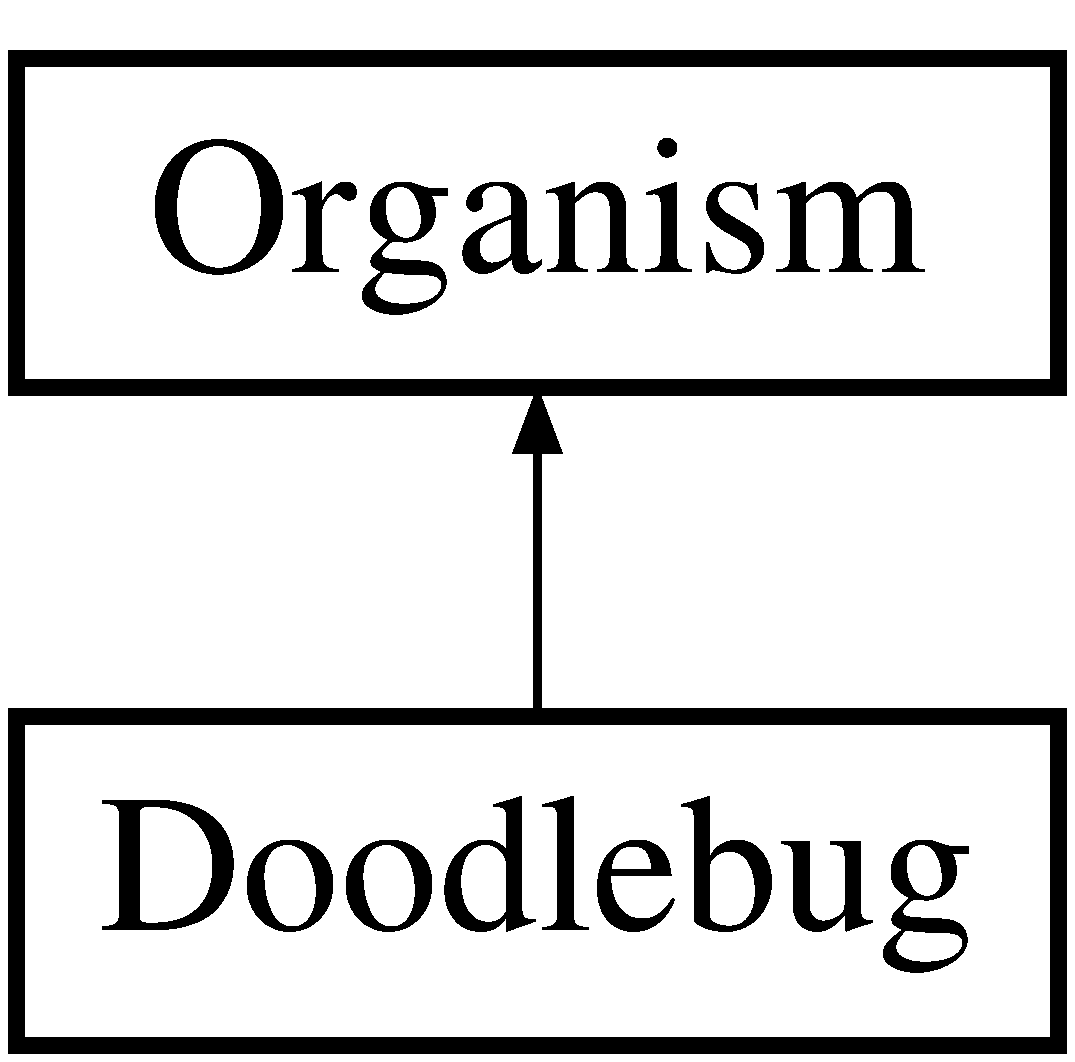
\includegraphics[height=2.000000cm]{classDoodlebug}
\end{center}
\end{figure}
\subsection*{Public Member Functions}
\begin{DoxyCompactItemize}
\item 
\textbf{ Doodlebug} ()
\item 
virtual \textbf{ $\sim$\+Doodlebug} ()
\item 
\textbf{ Doodlebug} (int \textbf{ x}, int \textbf{ y})
\item 
int \textbf{ get\+Time} ()
\item 
void \textbf{ move} ()
\item 
\textbf{ Doodlebug} $\ast$ \textbf{ breed} ()
\item 
bool \textbf{ is\+Move} (int \textbf{ x}, int \textbf{ y})
\item 
bool \textbf{ starve} ()
\item 
void \textbf{ action} ()
\item 
void \textbf{ simple\+Move} ()
\end{DoxyCompactItemize}
\subsection*{Private Attributes}
\begin{DoxyCompactItemize}
\item 
int \textbf{ hunger}
\end{DoxyCompactItemize}
\subsection*{Additional Inherited Members}


\subsection{Constructor \& Destructor Documentation}
\mbox{\label{classDoodlebug_afb2796ea39a6ffa13d4f54ac68dd52fc}} 
\index{Doodlebug@{Doodlebug}!Doodlebug@{Doodlebug}}
\index{Doodlebug@{Doodlebug}!Doodlebug@{Doodlebug}}
\subsubsection{Doodlebug()\hspace{0.1cm}{\footnotesize\ttfamily [1/2]}}
{\footnotesize\ttfamily Doodlebug\+::\+Doodlebug (\begin{DoxyParamCaption}{ }\end{DoxyParamCaption})}

\doxyref{Doodlebug()}{p.}{classDoodlebug_afb2796ea39a6ffa13d4f54ac68dd52fc} is the constructor for a \doxyref{Doodlebug}{p.}{classDoodlebug} object with no parameters 

Referenced by breed().

\mbox{\label{classDoodlebug_ac318cc9acbd9a3af52348a236070d891}} 
\index{Doodlebug@{Doodlebug}!````~Doodlebug@{$\sim$\+Doodlebug}}
\index{````~Doodlebug@{$\sim$\+Doodlebug}!Doodlebug@{Doodlebug}}
\subsubsection{$\sim$\+Doodlebug()}
{\footnotesize\ttfamily Doodlebug\+::$\sim$\+Doodlebug (\begin{DoxyParamCaption}{ }\end{DoxyParamCaption})\hspace{0.3cm}{\ttfamily [virtual]}}

\doxyref{$\sim$\+Doodlebug()}{p.}{classDoodlebug_ac318cc9acbd9a3af52348a236070d891} is the destructor for a \doxyref{Doodlebug}{p.}{classDoodlebug} object, it decrements the number of current doodlebugs 

References numD.

\mbox{\label{classDoodlebug_a19533236bfac6389c54a6559d5480fa4}} 
\index{Doodlebug@{Doodlebug}!Doodlebug@{Doodlebug}}
\index{Doodlebug@{Doodlebug}!Doodlebug@{Doodlebug}}
\subsubsection{Doodlebug()\hspace{0.1cm}{\footnotesize\ttfamily [2/2]}}
{\footnotesize\ttfamily Doodlebug\+::\+Doodlebug (\begin{DoxyParamCaption}\item[{int}]{x,  }\item[{int}]{y }\end{DoxyParamCaption})}

\doxyref{Doodlebug()}{p.}{classDoodlebug_afb2796ea39a6ffa13d4f54ac68dd52fc} is the constructor for a \doxyref{Doodlebug}{p.}{classDoodlebug} object with coordinates as parameters, and is initialized with default values. It increments the count of total and current doodlebugs 

References Organism\+::age, hunger, Organism\+::is\+Prey, numD, totalD, Organism\+::x, and Organism\+::y.



\subsection{Member Function Documentation}
\mbox{\label{classDoodlebug_a245518049f4a933c08fbd9e0c4d28be9}} 
\index{Doodlebug@{Doodlebug}!action@{action}}
\index{action@{action}!Doodlebug@{Doodlebug}}
\subsubsection{action()}
{\footnotesize\ttfamily void Doodlebug\+::action (\begin{DoxyParamCaption}{ }\end{DoxyParamCaption})\hspace{0.3cm}{\ttfamily [virtual]}}

\doxyref{action()}{p.}{classDoodlebug_a245518049f4a933c08fbd9e0c4d28be9} processes a regular turn of an ant, moving the ant and checking if it can breed in the current turn 

Implements \textbf{ Organism} \doxyref{}{p.}{classOrganism_af4dd34a96becf4f02ce4597901b81f60}.



References Organism\+::age, breed(), Organism\+::can\+Move, hunger, move(), starve(), totalD, Organism\+::x, and Organism\+::y.

\mbox{\label{classDoodlebug_a8b55bcada319ee2e9fc225073d9e72a2}} 
\index{Doodlebug@{Doodlebug}!breed@{breed}}
\index{breed@{breed}!Doodlebug@{Doodlebug}}
\subsubsection{breed()}
{\footnotesize\ttfamily \textbf{ Doodlebug} $\ast$ Doodlebug\+::breed (\begin{DoxyParamCaption}{ }\end{DoxyParamCaption})\hspace{0.3cm}{\ttfamily [virtual]}}

\doxyref{breed()}{p.}{classDoodlebug_a8b55bcada319ee2e9fc225073d9e72a2} checks the age of the doodlebug and creates a new doodlebug if the age of the doodlebug is at least 8. Upon creating a new doodlebug, moves it into an adjacent cell and resets the age of the current doodlebug

\begin{DoxyReturn}{Returns}
pointer to the newly born doodlebug or a null object if breeding conditions are not met 
\end{DoxyReturn}


Implements \textbf{ Organism} \doxyref{}{p.}{classOrganism_ad963420d8437f87bd8fe4277cc7f810a}.



References Organism\+::age, Doodlebug(), move(), totalD, Organism\+::x, and Organism\+::y.



Referenced by action().

\mbox{\label{classDoodlebug_a4325b77e742e8d1f93004f442f09461a}} 
\index{Doodlebug@{Doodlebug}!get\+Time@{get\+Time}}
\index{get\+Time@{get\+Time}!Doodlebug@{Doodlebug}}
\subsubsection{get\+Time()}
{\footnotesize\ttfamily int Doodlebug\+::get\+Time (\begin{DoxyParamCaption}{ }\end{DoxyParamCaption})\hspace{0.3cm}{\ttfamily [virtual]}}

\doxyref{get\+Time()}{p.}{classDoodlebug_a4325b77e742e8d1f93004f442f09461a} is a getter function for the turns which the doodlebug has been alive

\begin{DoxyReturn}{Returns}
age of the \doxyref{Doodlebug}{p.}{classDoodlebug} object 
\end{DoxyReturn}


Implements \textbf{ Organism} \doxyref{}{p.}{classOrganism_a9bc6dfde09d0e18a628cf843bb037d4b}.



References Organism\+::age.

\mbox{\label{classDoodlebug_ab5f01947b5eb3a92492162c2774344f9}} 
\index{Doodlebug@{Doodlebug}!is\+Move@{is\+Move}}
\index{is\+Move@{is\+Move}!Doodlebug@{Doodlebug}}
\subsubsection{is\+Move()}
{\footnotesize\ttfamily bool Doodlebug\+::is\+Move (\begin{DoxyParamCaption}\item[{int}]{x,  }\item[{int}]{y }\end{DoxyParamCaption})\hspace{0.3cm}{\ttfamily [virtual]}}

\doxyref{is\+Move()}{p.}{classDoodlebug_ab5f01947b5eb3a92492162c2774344f9} checks the state of the given cell to see whether the object can be moved into by an existing \doxyref{Doodlebug}{p.}{classDoodlebug}

\begin{DoxyReturn}{Returns}
a boolean for if the cell can be moved into 
\end{DoxyReturn}


Implements \textbf{ Organism} \doxyref{}{p.}{classOrganism_a7930747968e8533164d068be96f21ca0}.



Referenced by simple\+Move().

\mbox{\label{classDoodlebug_a75fb734381d7a316ba7370ba37c69471}} 
\index{Doodlebug@{Doodlebug}!move@{move}}
\index{move@{move}!Doodlebug@{Doodlebug}}
\subsubsection{move()}
{\footnotesize\ttfamily void Doodlebug\+::move (\begin{DoxyParamCaption}{ }\end{DoxyParamCaption})\hspace{0.3cm}{\ttfamily [virtual]}}

\doxyref{move()}{p.}{classDoodlebug_a75fb734381d7a316ba7370ba37c69471} checks the adjacent cells for prey, and attacks if it can. If it cannot, calls \doxyref{simple\+Move()}{p.}{classDoodlebug_a6b4ac6c11dc9b596eb6e83b245a43c2f} to move the the \doxyref{Doodlebug}{p.}{classDoodlebug} 

Implements \textbf{ Organism} \doxyref{}{p.}{classOrganism_a7fe2c98ea7b292d414b19bd67e885b55}.



References can\+Attack(), grid\+Len, hunger, on\+Edge(), simple\+Move(), Organism\+::x, and Organism\+::y.



Referenced by action(), breed(), and simple\+Move().

\mbox{\label{classDoodlebug_a6b4ac6c11dc9b596eb6e83b245a43c2f}} 
\index{Doodlebug@{Doodlebug}!simple\+Move@{simple\+Move}}
\index{simple\+Move@{simple\+Move}!Doodlebug@{Doodlebug}}
\subsubsection{simple\+Move()}
{\footnotesize\ttfamily void Doodlebug\+::simple\+Move (\begin{DoxyParamCaption}{ }\end{DoxyParamCaption})}

\doxyref{simple\+Move()}{p.}{classDoodlebug_a6b4ac6c11dc9b596eb6e83b245a43c2f} attempts to move a doodlebug into an adjacent cell, choosing one randomly and trying the rest. If none of the cases which were tried work, \doxyref{move()}{p.}{classDoodlebug_a75fb734381d7a316ba7370ba37c69471} calls itself recursively to try again. It also checks whether it is on the edge of the grid, and terminates if the ant is unable to move 

References grid\+Len, is\+Move(), move(), on\+Edge(), Organism\+::x, and Organism\+::y.



Referenced by move().

\mbox{\label{classDoodlebug_a7f1c26c8458f3811680c778362c0e374}} 
\index{Doodlebug@{Doodlebug}!starve@{starve}}
\index{starve@{starve}!Doodlebug@{Doodlebug}}
\subsubsection{starve()}
{\footnotesize\ttfamily bool Doodlebug\+::starve (\begin{DoxyParamCaption}{ }\end{DoxyParamCaption})}

\doxyref{starve()}{p.}{classDoodlebug_a7f1c26c8458f3811680c778362c0e374} checks the hunger of the doodlebug and kills off the doodlebug if the hunger conditions are met.

\begin{DoxyReturn}{Returns}
boolean indicating whether the doodlebug starved or not 
\end{DoxyReturn}


References hunger, Organism\+::x, and Organism\+::y.



Referenced by action().



\subsection{Member Data Documentation}
\mbox{\label{classDoodlebug_adf01154783c8192c8cc7ab194f22e542}} 
\index{Doodlebug@{Doodlebug}!hunger@{hunger}}
\index{hunger@{hunger}!Doodlebug@{Doodlebug}}
\subsubsection{hunger}
{\footnotesize\ttfamily int Doodlebug\+::hunger\hspace{0.3cm}{\ttfamily [private]}}



Referenced by action(), Doodlebug(), move(), and starve().



The documentation for this class was generated from the following files\+:\begin{DoxyCompactItemize}
\item 
\textbf{ Doodlebug.\+h}\item 
\textbf{ Doodlebug.\+cpp}\end{DoxyCompactItemize}

\section{Organism Class Reference}
\label{classOrganism}\index{Organism@{Organism}}


{\ttfamily \#include $<$Organism.\+h$>$}

Inheritance diagram for Organism\+:\begin{figure}[H]
\begin{center}
\leavevmode
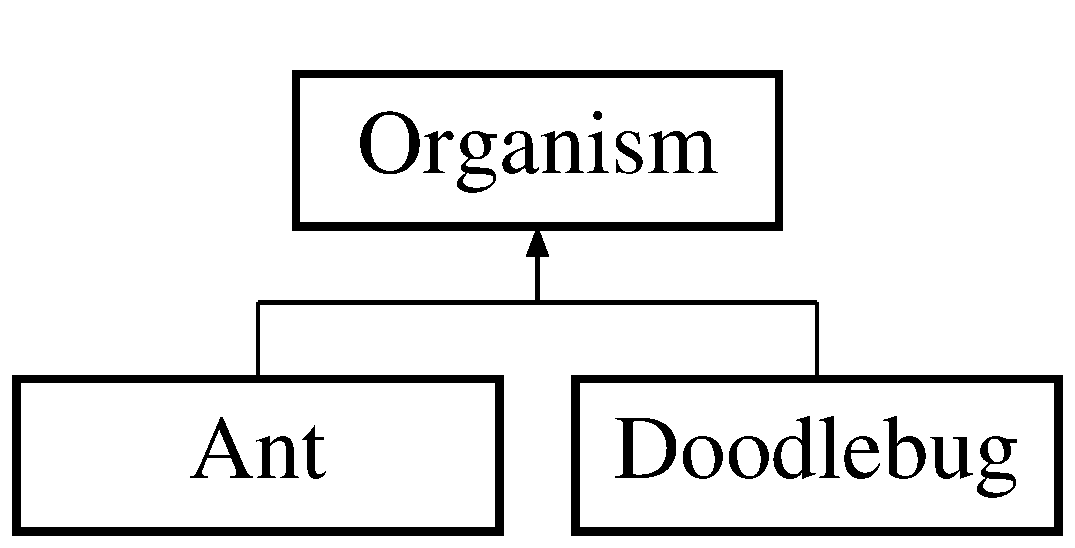
\includegraphics[height=2.000000cm]{classOrganism}
\end{center}
\end{figure}
\subsection*{Public Member Functions}
\begin{DoxyCompactItemize}
\item 
virtual int \textbf{ get\+Time} ()=0
\item 
virtual \textbf{ Organism} $\ast$ \textbf{ breed} ()=0
\item 
virtual void \textbf{ move} ()=0
\item 
virtual bool \textbf{ is\+Move} (int \textbf{ x}, int \textbf{ y})=0
\item 
virtual void \textbf{ action} ()=0
\item 
virtual \textbf{ $\sim$\+Organism} ()
\item 
\textbf{ Organism} ()
\end{DoxyCompactItemize}
\subsection*{Public Attributes}
\begin{DoxyCompactItemize}
\item 
int \textbf{ x}
\item 
int \textbf{ y}
\item 
int \textbf{ age}
\item 
bool \textbf{ is\+Prey}
\item 
bool \textbf{ can\+Move}
\end{DoxyCompactItemize}


\subsection{Constructor \& Destructor Documentation}
\mbox{\label{classOrganism_a35c0e3695065b80c5ad766c10ac441df}} 
\index{Organism@{Organism}!````~Organism@{$\sim$\+Organism}}
\index{````~Organism@{$\sim$\+Organism}!Organism@{Organism}}
\subsubsection{$\sim$\+Organism()}
{\footnotesize\ttfamily virtual Organism\+::$\sim$\+Organism (\begin{DoxyParamCaption}{ }\end{DoxyParamCaption})\hspace{0.3cm}{\ttfamily [inline]}, {\ttfamily [virtual]}}

\mbox{\label{classOrganism_aeb16ee24b64839584b4862384d0b53fe}} 
\index{Organism@{Organism}!Organism@{Organism}}
\index{Organism@{Organism}!Organism@{Organism}}
\subsubsection{Organism()}
{\footnotesize\ttfamily Organism\+::\+Organism (\begin{DoxyParamCaption}{ }\end{DoxyParamCaption})\hspace{0.3cm}{\ttfamily [inline]}}



\subsection{Member Function Documentation}
\mbox{\label{classOrganism_af4dd34a96becf4f02ce4597901b81f60}} 
\index{Organism@{Organism}!action@{action}}
\index{action@{action}!Organism@{Organism}}
\subsubsection{action()}
{\footnotesize\ttfamily virtual void Organism\+::action (\begin{DoxyParamCaption}{ }\end{DoxyParamCaption})\hspace{0.3cm}{\ttfamily [pure virtual]}}



Implemented in \textbf{ Doodlebug} \doxyref{}{p.}{classDoodlebug_a245518049f4a933c08fbd9e0c4d28be9}, and \textbf{ Ant} \doxyref{}{p.}{classAnt_a39fabe2c96298d5f7beb86649bf2dcab}.



Referenced by update().

\mbox{\label{classOrganism_ad963420d8437f87bd8fe4277cc7f810a}} 
\index{Organism@{Organism}!breed@{breed}}
\index{breed@{breed}!Organism@{Organism}}
\subsubsection{breed()}
{\footnotesize\ttfamily virtual \textbf{ Organism}$\ast$ Organism\+::breed (\begin{DoxyParamCaption}{ }\end{DoxyParamCaption})\hspace{0.3cm}{\ttfamily [pure virtual]}}



Implemented in \textbf{ Doodlebug} \doxyref{}{p.}{classDoodlebug_a8b55bcada319ee2e9fc225073d9e72a2}, and \textbf{ Ant} \doxyref{}{p.}{classAnt_a6829e25685f8a52a2acc38f5edbfc549}.

\mbox{\label{classOrganism_a9bc6dfde09d0e18a628cf843bb037d4b}} 
\index{Organism@{Organism}!get\+Time@{get\+Time}}
\index{get\+Time@{get\+Time}!Organism@{Organism}}
\subsubsection{get\+Time()}
{\footnotesize\ttfamily virtual int Organism\+::get\+Time (\begin{DoxyParamCaption}{ }\end{DoxyParamCaption})\hspace{0.3cm}{\ttfamily [pure virtual]}}



Implemented in \textbf{ Doodlebug} \doxyref{}{p.}{classDoodlebug_a4325b77e742e8d1f93004f442f09461a}, and \textbf{ Ant} \doxyref{}{p.}{classAnt_a39712b5c8852fcf2f0b7857e276e95c7}.

\mbox{\label{classOrganism_a7930747968e8533164d068be96f21ca0}} 
\index{Organism@{Organism}!is\+Move@{is\+Move}}
\index{is\+Move@{is\+Move}!Organism@{Organism}}
\subsubsection{is\+Move()}
{\footnotesize\ttfamily virtual bool Organism\+::is\+Move (\begin{DoxyParamCaption}\item[{int}]{x,  }\item[{int}]{y }\end{DoxyParamCaption})\hspace{0.3cm}{\ttfamily [pure virtual]}}



Implemented in \textbf{ Doodlebug} \doxyref{}{p.}{classDoodlebug_ab5f01947b5eb3a92492162c2774344f9}, and \textbf{ Ant} \doxyref{}{p.}{classAnt_a90943e89be8e68321ef0626e7770da59}.

\mbox{\label{classOrganism_a7fe2c98ea7b292d414b19bd67e885b55}} 
\index{Organism@{Organism}!move@{move}}
\index{move@{move}!Organism@{Organism}}
\subsubsection{move()}
{\footnotesize\ttfamily virtual void Organism\+::move (\begin{DoxyParamCaption}{ }\end{DoxyParamCaption})\hspace{0.3cm}{\ttfamily [pure virtual]}}



Implemented in \textbf{ Doodlebug} \doxyref{}{p.}{classDoodlebug_a75fb734381d7a316ba7370ba37c69471}, and \textbf{ Ant} \doxyref{}{p.}{classAnt_aaec1e3edaddd5e0ceedc333a9ac57a4c}.



\subsection{Member Data Documentation}
\mbox{\label{classOrganism_a571ad7154459ef315d9fe8706f77e300}} 
\index{Organism@{Organism}!age@{age}}
\index{age@{age}!Organism@{Organism}}
\subsubsection{age}
{\footnotesize\ttfamily int Organism\+::age}



Referenced by Ant\+::action(), Doodlebug\+::action(), Ant\+::\+Ant(), Ant\+::breed(), Doodlebug\+::breed(), Doodlebug\+::\+Doodlebug(), Ant\+::get\+Time(), and Doodlebug\+::get\+Time().

\mbox{\label{classOrganism_aa06754a444d1684c4df1e9d24cac63c0}} 
\index{Organism@{Organism}!can\+Move@{can\+Move}}
\index{can\+Move@{can\+Move}!Organism@{Organism}}
\subsubsection{can\+Move}
{\footnotesize\ttfamily bool Organism\+::can\+Move}



Referenced by Ant\+::action(), Doodlebug\+::action(), and update().

\mbox{\label{classOrganism_a9be19bc70a91f6200bc5e3ebe7b037e1}} 
\index{Organism@{Organism}!is\+Prey@{is\+Prey}}
\index{is\+Prey@{is\+Prey}!Organism@{Organism}}
\subsubsection{is\+Prey}
{\footnotesize\ttfamily bool Organism\+::is\+Prey}



Referenced by Ant\+::\+Ant(), can\+Attack(), and Doodlebug\+::\+Doodlebug().

\mbox{\label{classOrganism_a84f3cc4278086da52a0799c5409d124c}} 
\index{Organism@{Organism}!x@{x}}
\index{x@{x}!Organism@{Organism}}
\subsubsection{x}
{\footnotesize\ttfamily int Organism\+::x}



Referenced by Ant\+::action(), Doodlebug\+::action(), Ant\+::\+Ant(), Ant\+::breed(), Doodlebug\+::breed(), Doodlebug\+::\+Doodlebug(), Ant\+::is\+Move(), Ant\+::move(), Doodlebug\+::move(), Doodlebug\+::simple\+Move(), and Doodlebug\+::starve().

\mbox{\label{classOrganism_a3155ebae3b054a722cfbf8fdc68e3af6}} 
\index{Organism@{Organism}!y@{y}}
\index{y@{y}!Organism@{Organism}}
\subsubsection{y}
{\footnotesize\ttfamily int Organism\+::y}



Referenced by Ant\+::action(), Doodlebug\+::action(), Ant\+::\+Ant(), Ant\+::breed(), Doodlebug\+::breed(), Doodlebug\+::\+Doodlebug(), Ant\+::is\+Move(), Ant\+::move(), Doodlebug\+::move(), Doodlebug\+::simple\+Move(), and Doodlebug\+::starve().



The documentation for this class was generated from the following file\+:\begin{DoxyCompactItemize}
\item 
\textbf{ Organism.\+h}\end{DoxyCompactItemize}

\chapter{File Documentation}
\section{Ant.\+cpp File Reference}
\label{Ant_8cpp}\index{Ant.\+cpp@{Ant.\+cpp}}
{\ttfamily \#include \char`\"{}Ant.\+h\char`\"{}}\newline
{\ttfamily \#include $<$stdlib.\+h$>$}\newline
{\ttfamily \#include \char`\"{}main.\+h\char`\"{}}\newline
{\ttfamily \#include \char`\"{}Organism.\+h\char`\"{}}\newline
\subsection*{Variables}
\begin{DoxyCompactItemize}
\item 
\textbf{ Organism} $\ast$$\ast$$\ast$ \textbf{ grid}
\item 
int \textbf{ numA}
\item 
int \textbf{ totalA}
\item 
int \textbf{ grid\+Len}
\end{DoxyCompactItemize}


\subsection{Variable Documentation}
\mbox{\label{Ant_8cpp_aa32ee8a4e56a98f78518c23b635e5f69}} 
\index{Ant.\+cpp@{Ant.\+cpp}!grid@{grid}}
\index{grid@{grid}!Ant.\+cpp@{Ant.\+cpp}}
\subsubsection{grid}
{\footnotesize\ttfamily \textbf{ Organism}$\ast$$\ast$$\ast$ grid}

\mbox{\label{Ant_8cpp_a832020065060cfffc4a937e7b009b347}} 
\index{Ant.\+cpp@{Ant.\+cpp}!grid\+Len@{grid\+Len}}
\index{grid\+Len@{grid\+Len}!Ant.\+cpp@{Ant.\+cpp}}
\subsubsection{grid\+Len}
{\footnotesize\ttfamily int grid\+Len}



Referenced by Ant\+::move().

\mbox{\label{Ant_8cpp_ae5ad6ef3971548a3e89364353918967c}} 
\index{Ant.\+cpp@{Ant.\+cpp}!numA@{numA}}
\index{numA@{numA}!Ant.\+cpp@{Ant.\+cpp}}
\subsubsection{numA}
{\footnotesize\ttfamily int numA}



Referenced by Ant\+::\+Ant(), main(), and Ant\+::$\sim$\+Ant().

\mbox{\label{Ant_8cpp_a67d303aa718fb075f8c279ff737e7084}} 
\index{Ant.\+cpp@{Ant.\+cpp}!totalA@{totalA}}
\index{totalA@{totalA}!Ant.\+cpp@{Ant.\+cpp}}
\subsubsection{totalA}
{\footnotesize\ttfamily int totalA}



Referenced by Ant\+::\+Ant(), Ant\+::breed(), and main().


\section{Ant.\+h File Reference}
\label{Ant_8h}\index{Ant.\+h@{Ant.\+h}}
{\ttfamily \#include \char`\"{}Organism.\+h\char`\"{}}\newline
\subsection*{Classes}
\begin{DoxyCompactItemize}
\item 
class \textbf{ Ant}
\end{DoxyCompactItemize}

\section{Doodlebug.\+cpp File Reference}
\label{Doodlebug_8cpp}\index{Doodlebug.\+cpp@{Doodlebug.\+cpp}}
{\ttfamily \#include \char`\"{}Doodlebug.\+h\char`\"{}}\newline
{\ttfamily \#include $<$stdlib.\+h$>$}\newline
{\ttfamily \#include \char`\"{}Organism.\+h\char`\"{}}\newline
{\ttfamily \#include \char`\"{}main.\+h\char`\"{}}\newline
\subsection*{Variables}
\begin{DoxyCompactItemize}
\item 
\textbf{ Organism} $\ast$$\ast$$\ast$ \textbf{ grid}
\item 
int \textbf{ numD}
\item 
int \textbf{ totalD}
\item 
int \textbf{ grid\+Len}
\end{DoxyCompactItemize}


\subsection{Variable Documentation}
\mbox{\label{Doodlebug_8cpp_aa32ee8a4e56a98f78518c23b635e5f69}} 
\index{Doodlebug.\+cpp@{Doodlebug.\+cpp}!grid@{grid}}
\index{grid@{grid}!Doodlebug.\+cpp@{Doodlebug.\+cpp}}
\subsubsection{grid}
{\footnotesize\ttfamily \textbf{ Organism}$\ast$$\ast$$\ast$ grid}

\mbox{\label{Doodlebug_8cpp_a832020065060cfffc4a937e7b009b347}} 
\index{Doodlebug.\+cpp@{Doodlebug.\+cpp}!grid\+Len@{grid\+Len}}
\index{grid\+Len@{grid\+Len}!Doodlebug.\+cpp@{Doodlebug.\+cpp}}
\subsubsection{grid\+Len}
{\footnotesize\ttfamily int grid\+Len}



Referenced by main(), Doodlebug\+::move(), on\+Edge(), print\+Board(), Doodlebug\+::simple\+Move(), and update().

\mbox{\label{Doodlebug_8cpp_ad39b4dba918aab6239d9c16f42985b99}} 
\index{Doodlebug.\+cpp@{Doodlebug.\+cpp}!numD@{numD}}
\index{numD@{numD}!Doodlebug.\+cpp@{Doodlebug.\+cpp}}
\subsubsection{numD}
{\footnotesize\ttfamily int numD}



Referenced by Doodlebug\+::\+Doodlebug(), main(), and Doodlebug\+::$\sim$\+Doodlebug().

\mbox{\label{Doodlebug_8cpp_a52d67ee50023f4c10c59bcdc88ce6957}} 
\index{Doodlebug.\+cpp@{Doodlebug.\+cpp}!totalD@{totalD}}
\index{totalD@{totalD}!Doodlebug.\+cpp@{Doodlebug.\+cpp}}
\subsubsection{totalD}
{\footnotesize\ttfamily int totalD}



Referenced by Doodlebug\+::action(), Doodlebug\+::breed(), Doodlebug\+::\+Doodlebug(), and main().


\section{Doodlebug.\+h File Reference}
\label{Doodlebug_8h}\index{Doodlebug.\+h@{Doodlebug.\+h}}
{\ttfamily \#include \char`\"{}Organism.\+h\char`\"{}}\newline
\subsection*{Classes}
\begin{DoxyCompactItemize}
\item 
class \textbf{ Doodlebug}
\end{DoxyCompactItemize}

\section{main.\+cpp File Reference}
\label{main_8cpp}\index{main.\+cpp@{main.\+cpp}}
{\ttfamily \#include \char`\"{}Organism.\+h\char`\"{}}\newline
{\ttfamily \#include $<$stdlib.\+h$>$}\newline
{\ttfamily \#include $<$time.\+h$>$}\newline
{\ttfamily \#include \char`\"{}main.\+h\char`\"{}}\newline
{\ttfamily \#include \char`\"{}Doodlebug.\+h\char`\"{}}\newline
{\ttfamily \#include \char`\"{}Ant.\+h\char`\"{}}\newline
{\ttfamily \#include $<$iostream$>$}\newline
\subsection*{Functions}
\begin{DoxyCompactItemize}
\item 
bool \textbf{ on\+Edge} (int x, int y)
\item 
bool \textbf{ can\+Attack} (int x, int y)
\item 
void \textbf{ update} ()
\item 
void \textbf{ print\+Board} ()
\item 
int \textbf{ main} (int argc, char $\ast$$\ast$argv)
\end{DoxyCompactItemize}
\subsection*{Variables}
\begin{DoxyCompactItemize}
\item 
\textbf{ Organism} $\ast$$\ast$$\ast$ \textbf{ grid}
\item 
int \textbf{ numD}
\item 
int \textbf{ numA}
\item 
int \textbf{ totalD}
\item 
int \textbf{ totalA}
\item 
int \textbf{ grid\+Len}
\end{DoxyCompactItemize}


\subsection{Function Documentation}
\mbox{\label{main_8cpp_a61f1ac9e3f80b6f29b7b84e872c29117}} 
\index{main.\+cpp@{main.\+cpp}!can\+Attack@{can\+Attack}}
\index{can\+Attack@{can\+Attack}!main.\+cpp@{main.\+cpp}}
\subsubsection{can\+Attack()}
{\footnotesize\ttfamily bool can\+Attack (\begin{DoxyParamCaption}\item[{int}]{x,  }\item[{int}]{y }\end{DoxyParamCaption})}

\doxyref{can\+Attack()}{p.}{main_8cpp_a61f1ac9e3f80b6f29b7b84e872c29117} returns a boolean indicating whether the object in the given cell coordinates is able to attack

\begin{DoxyReturn}{Returns}
boolean indicating whether the given cell contains an organism which is able to attack 
\end{DoxyReturn}


References Organism\+::is\+Prey.



Referenced by Doodlebug\+::move().

\mbox{\label{main_8cpp_a3c04138a5bfe5d72780bb7e82a18e627}} 
\index{main.\+cpp@{main.\+cpp}!main@{main}}
\index{main@{main}!main.\+cpp@{main.\+cpp}}
\subsubsection{main()}
{\footnotesize\ttfamily int main (\begin{DoxyParamCaption}\item[{int}]{argc,  }\item[{char $\ast$$\ast$}]{argv }\end{DoxyParamCaption})}

\doxyref{main()}{p.}{main_8cpp_a3c04138a5bfe5d72780bb7e82a18e627} handles running the simulation, passing arguments initializing the grid, looping through eat step of the simulation, printing out the results, and then deallocating memory

\begin{DoxyReturn}{Returns}
0 for a successful program execution 
\end{DoxyReturn}


References grid\+Len, numA, numD, print\+Board(), totalA, totalD, and update().

\mbox{\label{main_8cpp_a341f5dc73f23bab79ca50e378ef4acef}} 
\index{main.\+cpp@{main.\+cpp}!on\+Edge@{on\+Edge}}
\index{on\+Edge@{on\+Edge}!main.\+cpp@{main.\+cpp}}
\subsubsection{on\+Edge()}
{\footnotesize\ttfamily bool on\+Edge (\begin{DoxyParamCaption}\item[{int}]{x,  }\item[{int}]{y }\end{DoxyParamCaption})}

\doxyref{on\+Edge()}{p.}{main_8cpp_a341f5dc73f23bab79ca50e378ef4acef} checks the cell which whose coordinates are passed and returns a boolean indicating whether it is on the edge of the grid or not

\begin{DoxyReturn}{Returns}
boolean indicating whether the given cell is on the edge 
\end{DoxyReturn}


References grid\+Len.



Referenced by Ant\+::move(), Doodlebug\+::move(), and Doodlebug\+::simple\+Move().

\mbox{\label{main_8cpp_a8310d6d1e915cb179f834d9ca017950a}} 
\index{main.\+cpp@{main.\+cpp}!print\+Board@{print\+Board}}
\index{print\+Board@{print\+Board}!main.\+cpp@{main.\+cpp}}
\subsubsection{print\+Board()}
{\footnotesize\ttfamily void print\+Board (\begin{DoxyParamCaption}{ }\end{DoxyParamCaption})}

\doxyref{print\+Board()}{p.}{main_8cpp_a8310d6d1e915cb179f834d9ca017950a} loops through the grid, printing out the current state of the grid with x\textquotesingle{}s indicating a doodlebug and o\textquotesingle{}s indicating an ant 

References grid\+Len.



Referenced by main().

\mbox{\label{main_8cpp_ac5c54df7ed3b930268c8d7752c101725}} 
\index{main.\+cpp@{main.\+cpp}!update@{update}}
\index{update@{update}!main.\+cpp@{main.\+cpp}}
\subsubsection{update()}
{\footnotesize\ttfamily void update (\begin{DoxyParamCaption}{ }\end{DoxyParamCaption})}

\doxyref{update()}{p.}{main_8cpp_ac5c54df7ed3b930268c8d7752c101725} loops through the grid, updating can\+Move for all organisms and then updates all organisms on the grid, updating all doodlebugs first and all ants 

References Organism\+::action(), Organism\+::can\+Move, and grid\+Len.



Referenced by main().



\subsection{Variable Documentation}
\mbox{\label{main_8cpp_aa32ee8a4e56a98f78518c23b635e5f69}} 
\index{main.\+cpp@{main.\+cpp}!grid@{grid}}
\index{grid@{grid}!main.\+cpp@{main.\+cpp}}
\subsubsection{grid}
{\footnotesize\ttfamily \textbf{ Organism}$\ast$$\ast$$\ast$ grid}

\mbox{\label{main_8cpp_a832020065060cfffc4a937e7b009b347}} 
\index{main.\+cpp@{main.\+cpp}!grid\+Len@{grid\+Len}}
\index{grid\+Len@{grid\+Len}!main.\+cpp@{main.\+cpp}}
\subsubsection{grid\+Len}
{\footnotesize\ttfamily int grid\+Len}



Referenced by main(), Ant\+::move(), Doodlebug\+::move(), on\+Edge(), print\+Board(), Doodlebug\+::simple\+Move(), and update().

\mbox{\label{main_8cpp_ae5ad6ef3971548a3e89364353918967c}} 
\index{main.\+cpp@{main.\+cpp}!numA@{numA}}
\index{numA@{numA}!main.\+cpp@{main.\+cpp}}
\subsubsection{numA}
{\footnotesize\ttfamily int numA}



Referenced by Ant\+::\+Ant(), main(), and Ant\+::$\sim$\+Ant().

\mbox{\label{main_8cpp_ad39b4dba918aab6239d9c16f42985b99}} 
\index{main.\+cpp@{main.\+cpp}!numD@{numD}}
\index{numD@{numD}!main.\+cpp@{main.\+cpp}}
\subsubsection{numD}
{\footnotesize\ttfamily int numD}



Referenced by Doodlebug\+::\+Doodlebug(), main(), and Doodlebug\+::$\sim$\+Doodlebug().

\mbox{\label{main_8cpp_a67d303aa718fb075f8c279ff737e7084}} 
\index{main.\+cpp@{main.\+cpp}!totalA@{totalA}}
\index{totalA@{totalA}!main.\+cpp@{main.\+cpp}}
\subsubsection{totalA}
{\footnotesize\ttfamily int totalA}



Referenced by Ant\+::\+Ant(), Ant\+::breed(), and main().

\mbox{\label{main_8cpp_a52d67ee50023f4c10c59bcdc88ce6957}} 
\index{main.\+cpp@{main.\+cpp}!totalD@{totalD}}
\index{totalD@{totalD}!main.\+cpp@{main.\+cpp}}
\subsubsection{totalD}
{\footnotesize\ttfamily int totalD}



Referenced by Doodlebug\+::action(), Doodlebug\+::breed(), Doodlebug\+::\+Doodlebug(), and main().


\section{main.\+h File Reference}
\label{main_8h}\index{main.\+h@{main.\+h}}
{\ttfamily \#include \char`\"{}Organism.\+h\char`\"{}}\newline
\subsection*{Functions}
\begin{DoxyCompactItemize}
\item 
bool \textbf{ on\+Edge} (int x, int y)
\item 
bool \textbf{ can\+Attack} (int x, int y)
\end{DoxyCompactItemize}


\subsection{Function Documentation}
\mbox{\label{main_8h_a61f1ac9e3f80b6f29b7b84e872c29117}} 
\index{main.\+h@{main.\+h}!can\+Attack@{can\+Attack}}
\index{can\+Attack@{can\+Attack}!main.\+h@{main.\+h}}
\subsubsection{can\+Attack()}
{\footnotesize\ttfamily bool can\+Attack (\begin{DoxyParamCaption}\item[{int}]{x,  }\item[{int}]{y }\end{DoxyParamCaption})}

\doxyref{can\+Attack()}{p.}{main_8cpp_a61f1ac9e3f80b6f29b7b84e872c29117} returns a boolean indicating whether the object in the given cell coordinates is able to attack

\begin{DoxyReturn}{Returns}
boolean indicating whether the given cell contains an organism which is able to attack 
\end{DoxyReturn}


References Organism\+::is\+Prey.



Referenced by Doodlebug\+::move().

\mbox{\label{main_8h_a341f5dc73f23bab79ca50e378ef4acef}} 
\index{main.\+h@{main.\+h}!on\+Edge@{on\+Edge}}
\index{on\+Edge@{on\+Edge}!main.\+h@{main.\+h}}
\subsubsection{on\+Edge()}
{\footnotesize\ttfamily bool on\+Edge (\begin{DoxyParamCaption}\item[{int}]{x,  }\item[{int}]{y }\end{DoxyParamCaption})}

\doxyref{on\+Edge()}{p.}{main_8cpp_a341f5dc73f23bab79ca50e378ef4acef} checks the cell which whose coordinates are passed and returns a boolean indicating whether it is on the edge of the grid or not

\begin{DoxyReturn}{Returns}
boolean indicating whether the given cell is on the edge 
\end{DoxyReturn}


References grid\+Len.



Referenced by Ant\+::move(), Doodlebug\+::move(), and Doodlebug\+::simple\+Move().


\section{Organism.\+cpp File Reference}
\label{Organism_8cpp}\index{Organism.\+cpp@{Organism.\+cpp}}
{\ttfamily \#include \char`\"{}Organism.\+h\char`\"{}}\newline
{\ttfamily \#include \char`\"{}main.\+h\char`\"{}}\newline

\section{Organism.\+h File Reference}
\label{Organism_8h}\index{Organism.\+h@{Organism.\+h}}
{\ttfamily \#include $<$stdlib.\+h$>$}\newline
{\ttfamily \#include \char`\"{}main.\+h\char`\"{}}\newline
\subsection*{Classes}
\begin{DoxyCompactItemize}
\item 
class \textbf{ Organism}
\end{DoxyCompactItemize}

%--- End generated contents ---

% Index
\backmatter
\newpage
\phantomsection
\clearemptydoublepage
\addcontentsline{toc}{chapter}{Index}
\printindex

\end{document}
